\documentclass[12pt,a4paper,openright,twoside]{book}

%pacchetti vari
\usepackage[italian]{babel} 	%per l'italiano
\usepackage[T1]{fontenc}		%per vedere lettere accentate
\usepackage[utf8]{inputenc}		%per inserire lettere accentate
\usepackage{textcomp}			%boh
\usepackage{floatflt}			%immagini fluttuanti
\usepackage{frontespizio}
\usepackage[font=small,hang]{caption} %caption delle immagini
\usepackage{graphicx}	%boh
\usepackage{hyperref}	%per i link
\usepackage{fullpage}
\usepackage{chngcntr}
\counterwithout{footnote}{chapter}
\usepackage{subfig}

\begin{document}
    
    \tableofcontents %indice
    \newpage
    \thispagestyle{empty}
    \chapter*{Introduzione}
    \addcontentsline{toc}{chapter}{Introduzione}
    Questa tesi ha l'obiettivo di illustrare il lavoro svolto per sviluppare un videogioco il cui principio è quello di 
    fornire uno strumento per il trattamento dell'ambliopia anche nel tempo libero. Infatti, come si mostrerà in seguito, un fattore 
    importante per la creazione del videogioco mostrato nei capitoli seguenti, è quello di far congiungere la terapia
    con il divertimento.  \\\\
    Il nome del videogioco è Clash Ninja ed è da considerarsi una parte del progetto \textsc{3D4Amb} (sito ufficiale, \url{https://3d4amb.unibg.it}) dell'Università degli Studi di Bergamo supervisionato dal prof. Angelo Gargantini. \\\\
    Per prima cosa si farà un'analisi del contesto, ovvero in cosa consiste l'ambliopia, come viene causata e come viene
    trattata indicando le varie tecniche per poter combattere tale patologia.\\\\
    Si parlerà inoltre del progetto 3D4Amb indicando come esso intende affrontare il problema sfruttando diverse tecnologie e 
    esponendo i requisiti richiesti per rendere il videogioco conforme alla sua filosofia.\\\\
    Verranno riportati gli strumenti utilizzati per lo sviluppo e la scelta degli accessori per testare il videogioco. \\\\
    Infine si espone il lavoro svolto per lo sviluppo software di Clash Ninja descrivendone le tecniche utilizzate e gli elementi
    del videogioco.
    
    \newpage  
    \thispagestyle{empty}
    
    
    \chapter{Ambliopia}
    \section{Cos'è l'ambliopia?}
    L'ambliopia è una malattia degli occhi e dell'apparato visivo estremamente frequente e pericolosa che colpisce soggetti in età pediatrica.
    Il termine deriva dal greco e, più esattamente, da "ops" (che significa "visione") e "amblyos" (che significa "ottusa, pigra"). Il suo nome comune è "occhio pigro". \cite{wiki:xxx} \\ Essa è una condizione in cui la funzione visiva di un occhio è ridotta o assente senza che ci siano stati danni oculari organici e consiste in un deficit dell’apparato visivo : il cervello, non riuscendo a interpretare correttamente le informazioni che gli giungono, “disattiva” i segnali che provengono da un occhio. \cite{iapbamb} \\
    
    \section{Cause dell'ambliopia}
    Le cause più comuni dell'ambliopia sono:
    \begin{itemize}
    	\item Lo strabismo, cioè un anomalo allineamento degli occhi, provocato da un difetto dei meccanismi neuro-muscolari che ne controllano i movimenti;
    	\item Cataratta congenita e ptosi palpebrale;
    	\item Astigmatismo e ipermetropia se non vengono corretti adeguatamente e tempestivamente;
    	\item Anisometropia, cioè una differente refrazione tra i due occhi. \cite{humamb}
    \end{itemize}
	Si rileva quindi l'importanza di diagnosticare l'ambliopia già in età pediatrica, poichè è la fase con maggior reversibilità e possibilità di curare la patologia. Infatti ne è affetto circa il 4-5\% tra i pazienti in età pediatrica e circa il 2\% in età adulta, ciò 
	perchè il trattamento avviene spesso nell'infanzia.
	\section{Tipologie di ambliopia}
	\subsection{Ambliopia anisometropica}
	In questo caso l'ambliopia è sostenuta da una differenza di refrazione\footnote{Fenomeno di deviazione di un onda quando passa da un mezzo ad un altro.} fra i due occhi. In molti casi vi è un occhio sano e l'altro con problemi di astigmatismo o ipermetropia, ma vi sono anche casi in cui entrambi gli occhi hanno difetti di refrazione di diversa entità fra loro.
	La conseguenza è che l'occhio buono o quello con minor difetto di refrazione viene utilizzato molto
	più dell'altro e così quest'ultimo,se non adeguatamente corretto o stimolato, viene usato molto meno
	andando incontro all'ambliopia.
	La terapia dell'ambliopia anisometropica è la stessa usata per la terapia dell'ambliopia strabica.  \cite{strabpedr}
	\subsection{Ambliopia strabica} 
	L'ambliopia strabica è la più riscontrata tra i pazienti: si manifesta infatti nel 35-50\% dei casi di strabismo. Il fattore ambliopigeno è dato dalla deviazione oculare costante o comunque presente per la
	maggior parte della giornata. \\
	Non esiste alcuna relazione fra entità della deviazione e gravità dell’ambliopia: un microstrabismo
	può comunque provocare l’insorgenza di una ambliopia importante. 
    \section{Diagnosi dell'ambliopia}
    I sintomi dell'ambliopia spesso non vengono percepiti in quanto i pazienti sono piccoli. Pertanto è importante ricorrere a visite oculistiche alla nascita, ad un anno di età ed un ulteriore controllo intorno ai 2-3 anni di età poichè si è nella fase in 
    cui è possibile rilevare l'acuità visiva. In caso di strabismo occorre anche una visita ortottica.
    \section{Trattamenti}
    Esistono diversi trattamenti dell'ambliopia, che presentano metodologie diverse, ma si basano sul concetto di penalizzare la percezione dell'occhio sano favorendo così l'utilizzo dell'occhio malato. Ciò permette di "ristimolare" il cervello a elaborare le informazioni 
    provenienti dall'occhio malato. I trattamenti più diffusi sono:
    \begin{itemize}
    	\item Metodo occlusivo;
    	\item Atropina;
    	\item Metodo I-BiT;
    \end{itemize}
    \subsection{Metodo occlusivo}
  
	 Il metodo occlusivo è il più conosciuto e utilizzato trattamento per l'ambliopia. Come raffigurato nella \figurename \ref{fig:metoccl},
	 esso consiste nell'applicare un bendaggio occlusivo sull'occhio sano per un certo numero di ore. Ciò rende disponibile solo l'occhio 
	 ambliope in modo da forzare il cervello a elaborare le informazioni provenienti da tale occhio che normalmente viene ignorato.\\
	 Le possibilità di successo della terapia con la benda occlusiva è legato all'età del paziente: più l'età è bassa e più vi è probabilità che con tale metodo si elimini (anche parzialmente) il problema dell'ambliopia.\\
	 L'occlusione è un trattamento molto semplice e poco costoso, ma nel periodo di applicazione del bendaggio il paziente ha a disposizione un solo occhio per avere un impatto visivo dell'ambiente circostante. Ciò può comportare dei disorientamenti.\\
	 È richiesto un controllo periodico dei miglioramenti (solitamente si visita il paziente ogni 6-7 settimane) per definire le ore giornaliere e la lunghezza del periodo in cui il paziente dovrà 
	 tenere la benda sull'occhio.\\
	  \begin{figure}[h]
	 	\centering   	
	 	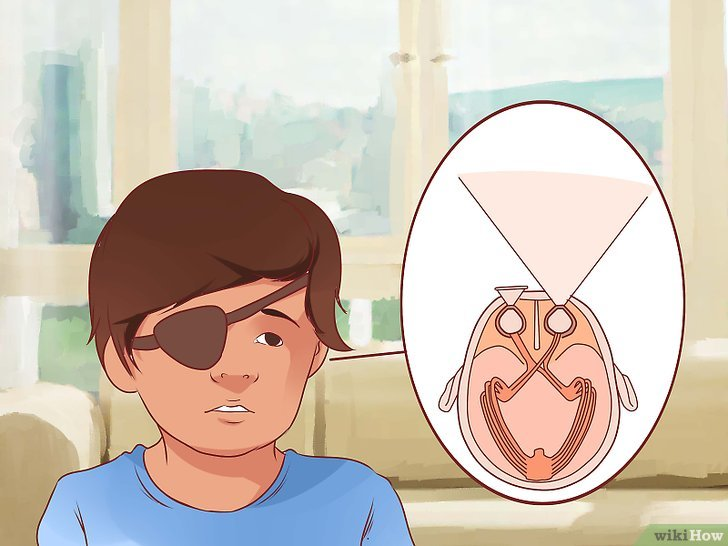
\includegraphics[width=60mm]{metoccl.jpg}
	 	\caption{Bendaggio occlusivo sull'occhio sano}
	 	\label{fig:metoccl}
	 \end{figure}
    \subsection{Atropina}
    Un' alternativa all'occlusione tramite un bendaggio vi è la penalizzazione farmacologica dell'occhio sano tramite una somministrazione di atropina.\\
    L'atropina è un tropan-alcaloide\footnote{famiglia di alcaloidi che contengono un anello tropanico nella loro struttura chimica.} impiegato per la produzione di un particolare collirio in grado di provocare la dilatazione della pupilla, effetto richiesto in occasione di interventi diagnostici e chirurgici sull'occhio, nonché nel trattamento di alcune malattie infiammatorie dell'occhio.\\
    Nel caso di ambliopia, la penalizzazione farmacologica mediante l'impiego di atropina impedisce l’accomodazione dell’occhio buono, promuovendo così l'utilizzo dell'occhio ambliope per oggetti vicini.\\
    Inizialmente questa terapia è stata utilizzata per ambliopia lieve poichè è stata giudicata insufficiente per il miglioramento di ambliopie più gravi. Recentemente però, attraverso studi scientifici, è stato dimostrato che la cura attraverso la dilatazione della pupilla porta notevoli progressi anche in casi di ambliopie importanti.
    \begin{figure}[h]
    	\centering   	
    	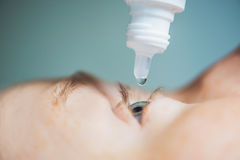
\includegraphics[width=60mm]{atrop.jpg}
    	\caption{Somministrazione di atropina sull'occhio sano}
    	\label{fig:atrop}
    \end{figure}
\newpage
    \subsection{Metodo I-BiT}
    University of Notthingham ha in corso un progetto per il trattamento dell'ambliopia indirizzato soprattutto per i pazienti più giovani: il progetto I-BiT (Interactive Binocular Treatment for Amblyopia).\\
    I-BiT consiste nello sviluppo di videogiochi interattivi basati sulla realtà virtuale, i quali devono avere i seguenti requisiti: 
    \begin{itemize}
    	\item Gli elementi secondari del gioco devono essere mostrati all'occhio sano;
    	\item Gli elementi principali del gioco devono essere mostrati esclusivamente all'occhio ambliope.
    \end{itemize}
	Ciò favorisce quindi di sfruttare di più le informazioni provenienti dall'occhio ambliope per avanzare nel videogioco.\\
	I-BiT è un metodo non ancora molto diffuso per via delle dimensioni ingombranti e degli elevati costi delle apparecchiature.
     \begin{figure}[h]
    	\centering   	
    	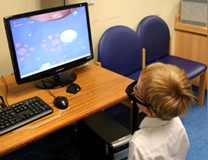
\includegraphics[width=60mm]{i-bit.jpg}
    	\caption{Un bambino sottoposto al metodo I-BiT}
    	\label{fig:ibit}
    \end{figure}
    \chapter{3D4Amb}
    \section{Introduzione al progetto}
    3D4Amb è un progetto sviluppato dall'Università degli Studi di Bergamo che mira alla creazione di sistemi basati sulla tecnologia 3D active shutter\footnote{Tecnologia che consente di visualizzare immagini stereoscopiche 3D} per la diagnosi e il trattamento dell'ambliopia soprattutto nei bambini.\\
    La tecnologia 3D active shutter viene sfuttata per fornire una visione binoculare, ovvero mostrare immagini diverse all'occhio sano da quello ambliope. Ciò consente di effettuare diagnosi e trattamenti dell'ambliopia mediante giochi interattivi e attività di intrattenimento.\\
    Il progetto è coordinato dal prof. Angelo Gargantini con la collaborazione del Centro di ipovisione e riabilitazione visiva degli Ospedali Riuniti di Bergamo, del Policlinico di Milano e dell'Università degli Studi di Milano.
    
     \begin{figure}[h]
    	\centering   	
    	
\includegraphics[width=60mm]{logo3d4amb.png}
    	\caption{Logo ufficiale di 3D4Amb}
    	\label{fig:3d4amb}
    \end{figure}
    \section{Obiettivo del progetto}
    Come introdotto nel paragrafo precedente, 3D4Amb mira al svillupo di sistemi per la diagnosi e il trattamento dell'ambliopia. I principi fondamentali di tali sistemi, secondo le specifiche di 3D4Amb, devono essere:
    \begin{enumerate}
    	\item \textbf{\textit{Economicità}}: Il sistema deve poter essere utilizzato anche mediante l'uso di attrezzature e dispositivi poco costosi;
    	\item \textbf{\textit{Comodità}}: l'utilizzo del sistema può avvenire in qualsiasi ambiente e non per forza in centri specializzati o negli ospedali;
    	\item \textbf{\textit{Usabilità}}: Il sistema deve poter essere utilizzato facilmente da qualsiasi utente (soprattutto bambini);
    	\item \textbf{\textit{Divertimento}}: Il sistema deve trasmettere intrattenimento all'utente che lo sta utilizzando, alimentando così la propensione dell'utente a collaborare. Ciò facilizza il successo della diagnosi e del trattamento dell'ambliopia. 
    \end{enumerate}
	Con i metodi tradizionali capita spesso che ci sia poco coinvolgimento da parte dei pazienti in età pediatrica e ciò può portare ad avere ben pochi miglioramenti nella terapia. Perciò è importante poter congiungere il trattamento con l'intrattenimento.

    \section{Tecniche}
    \subsection{Tecnica con anaglifi}
    L'anaglifo è un immagine stereoscopica che, se osservata con appositi occhiali (come quelli in \figurename \ref{fig:anagl}), fornisce un illusione di tridimensionalità.\\
    Per creare un immagine anaglifica vengono riprese due immagini parallele alla distanza degli occhi umani. Una delle due immagini viene filtrata con il colore rosso (che è un colore sottrattivo) mentre l'altra viene filtrata con un filtro complementare (come il ciano, il blu e il verde che sono colori additivi). Infine si uniscono le due immagini e si stampa l'anaglifo, oppure è possibile proiettare le due immagini simultaneamente.\\ Visualizzare l'anaglifo a occhio nudo però non è agevole e non si percepisce l'illusione della tridimensionalità. Se però si visualizza l'immagine con appositi occhiali dove si ha una lente rossa e una lente filtrata con un colore additivo si percepisce una profondità dell'immagine che in realtà non esiste: l'occhio che vede attraverso il filtro rosso vedrà le parti di immagine rosse come parti "chiare", mentre l'occhio che vede attraverso il filtro ciano scarta le parti rosse e vede le parti dell'immagine ciano come parti "scure", così da fornire la tridimensionalità dell'immagine. 
    \begin{figure}[h]
    	\centering
    	 \subfloat{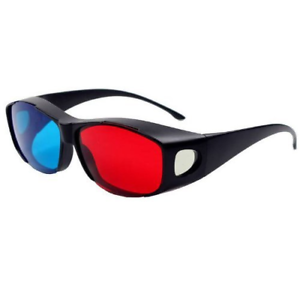
\includegraphics[width=.45\columnwidth]{anaglif.png}} \quad
    	\subfloat{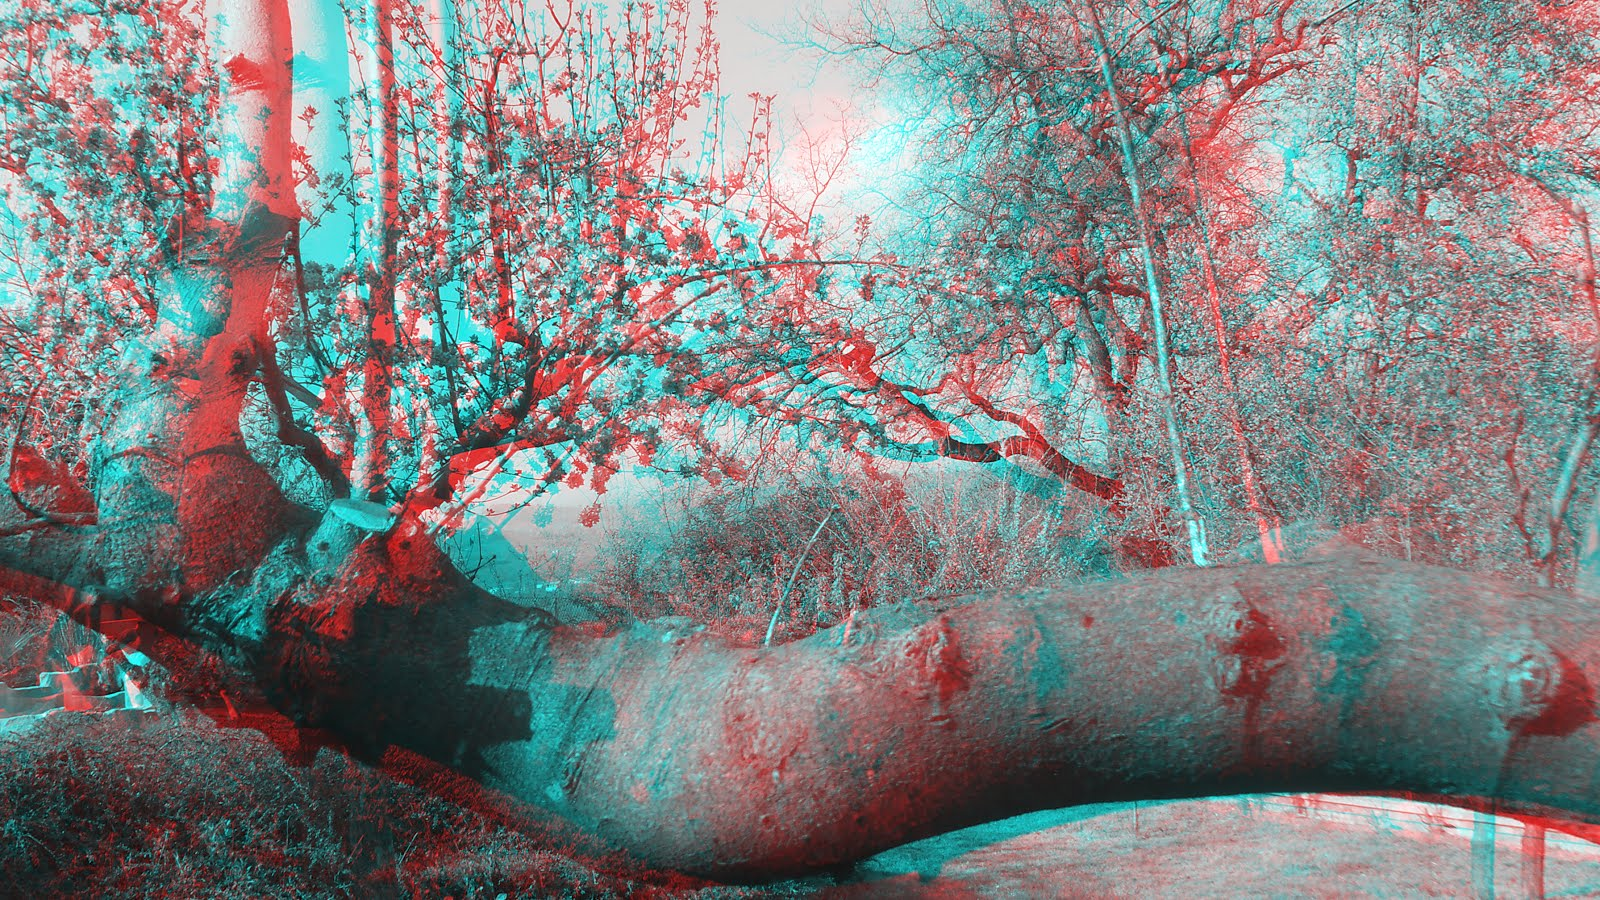
\includegraphics[width=.45\columnwidth]{ramanag.jpg}}
    	\caption{A sinistra occhiali per anaglifi. A destra immagine trasformata in anaglifo}
    	\label{fig:anagl}
    \end{figure}
\newpage
    \subsection{Tecnica con gli occhiali 3D}
     \begin{figure}[h]
    	\centering   	
    	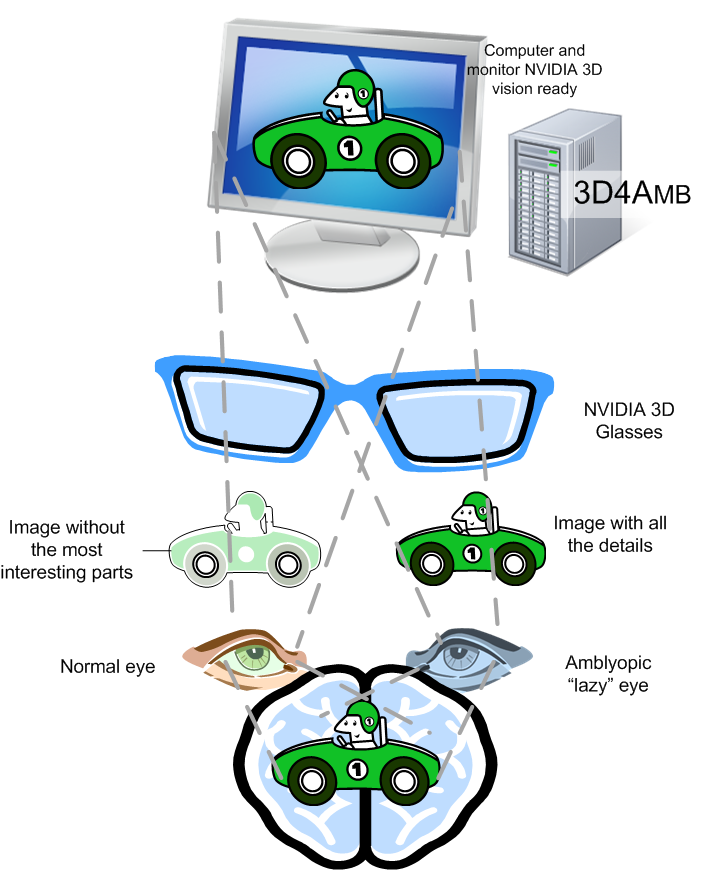
\includegraphics[width=10cm, height=12cm]{visione.png}
    	\caption{Utilizzo della tecnologia 3D in 3D4Amb}
    	\label{fig:visione}
    \end{figure}
	\subsection{Tecnica con headset VR}
	\chapter{Clash Ninja: Studi preliminari} 
	\chapter{Clash Ninja: Realizzazione}   
    \bibliographystyle{plain}
    \bibliography{BibliografiaTesi}
\end{document}